% Workshop-style draft. Every number is a macro generated from results/metrics.json by
% src/report.py (see numbers.tex). To submit, move the body into the official ACL or
% NeurIPS workshop template; the content is template-independent.
\documentclass[10pt,twocolumn]{article}
\usepackage[letterpaper,margin=0.75in,columnsep=0.25in]{geometry}
\usepackage{newtxtext,newtxmath}
\usepackage[T1]{fontenc}
\usepackage{graphicx}
\usepackage{booktabs}
\usepackage{xcolor}
\usepackage[numbers,sort&compress]{natbib}
\usepackage[hidelinks]{hyperref}
\usepackage{caption}
\captionsetup{font=small,labelfont=bf}
\setlength{\tabcolsep}{4pt}

% AUTO-GENERATED by src/report.py from results/metrics.json. Do not edit.
\newcommand{\GpuSevenMin}{26}
\newcommand{\GpuThreeMin}{15}
\newcommand{\PilotN}{100}
\newcommand{\PmAcc}{61.6}
\newcommand{\PmAccAll}{62.2}
\newcommand{\PmAccCI}{58.7--64.4}
\newcommand{\PmAucAnsId}{0.753}
\newcommand{\PmAucLogProb}{0.731}
\newcommand{\PmAucProbeAns}{0.839}
\newcommand{\PmAucProbePrompt}{0.830}
\newcommand{\PmAucSCfive}{0.669}
\newcommand{\PmAucSCten}{0.698}
\newcommand{\PmAucSEfive}{0.671}
\newcommand{\PmAucSEten}{0.701}
\newcommand{\PmAucSEtenLen}{0.702}
\newcommand{\PmAuracAnsId}{0.787}
\newcommand{\PmAuracLogProb}{0.782}
\newcommand{\PmAuracProbeAns}{0.839}
\newcommand{\PmAuracProbePrompt}{0.838}
\newcommand{\PmAuracSCfive}{0.719}
\newcommand{\PmAuracSCten}{0.744}
\newcommand{\PmAuracSEfive}{0.720}
\newcommand{\PmAuracSEten}{0.745}
\newcommand{\PmAuracSEtenLen}{0.745}
\newcommand{\PmCiAnsId}{[0.708, 0.794]}
\newcommand{\PmCiLogProb}{[0.685, 0.775]}
\newcommand{\PmCiProbeAns}{[0.800, 0.873]}
\newcommand{\PmCiProbePrompt}{[0.791, 0.864]}
\newcommand{\PmCiSCfive}{[0.624, 0.712]}
\newcommand{\PmCiSCten}{[0.649, 0.741]}
\newcommand{\PmCiSEfive}{[0.624, 0.715]}
\newcommand{\PmCiSEten}{[0.652, 0.745]}
\newcommand{\PmCiSEtenLen}{[0.655, 0.747]}
\newcommand{\PmDCiProbeAnsvsAnsId}{[+0.053, +0.117]}
\newcommand{\PmDCiProbeAnsvsLogProb}{[+0.059, +0.156]}
\newcommand{\PmDCiProbeAnsvsSCfive}{[+0.119, +0.218]}
\newcommand{\PmDCiProbeAnsvsSCten}{[+0.094, +0.189]}
\newcommand{\PmDCiProbeAnsvsSEfive}{[+0.118, +0.216]}
\newcommand{\PmDCiProbeAnsvsSEten}{[+0.090, +0.186]}
\newcommand{\PmDCiProbeAnsvsSEtenLen}{[+0.087, +0.187]}
\newcommand{\PmDCiProbePromptvsAnsId}{[+0.037, +0.116]}
\newcommand{\PmDCiProbePromptvsLogProb}{[+0.056, +0.145]}
\newcommand{\PmDCiProbePromptvsSCfive}{[+0.113, +0.206]}
\newcommand{\PmDCiProbePromptvsSCten}{[+0.087, +0.178]}
\newcommand{\PmDCiProbePromptvsSEfive}{[+0.110, +0.205]}
\newcommand{\PmDCiProbePromptvsSEten}{[+0.084, +0.175]}
\newcommand{\PmDCiProbePromptvsSEtenLen}{[+0.082, +0.172]}
\newcommand{\PmDProbeAnsvsAnsId}{+0.085}
\newcommand{\PmDProbeAnsvsLogProb}{+0.108}
\newcommand{\PmDProbeAnsvsSCfive}{+0.170}
\newcommand{\PmDProbeAnsvsSCten}{+0.141}
\newcommand{\PmDProbeAnsvsSEfive}{+0.168}
\newcommand{\PmDProbeAnsvsSEten}{+0.138}
\newcommand{\PmDProbeAnsvsSEtenLen}{+0.136}
\newcommand{\PmDProbePromptvsAnsId}{+0.077}
\newcommand{\PmDProbePromptvsLogProb}{+0.099}
\newcommand{\PmDProbePromptvsSCfive}{+0.162}
\newcommand{\PmDProbePromptvsSCten}{+0.133}
\newcommand{\PmDProbePromptvsSEfive}{+0.159}
\newcommand{\PmDProbePromptvsSEten}{+0.129}
\newcommand{\PmDProbePromptvsSEtenLen}{+0.128}
\newcommand{\PmFpAnsId}{2.0}
\newcommand{\PmFpLogProb}{2.0}
\newcommand{\PmFpProbeAns}{2.0}
\newcommand{\PmFpProbePrompt}{1.0}
\newcommand{\PmFpSCfive}{12.0}
\newcommand{\PmFpSCten}{22.0}
\newcommand{\PmFpSEfive}{12.9}
\newcommand{\PmFpSEten}{23.2}
\newcommand{\PmFpSEtenLen}{23.3}
\newcommand{\PmGoldMaybePct}{11}
\newcommand{\PmHalfAccAnsId}{77.3}
\newcommand{\PmHalfAccLogProb}{77.2}
\newcommand{\PmHalfAccProbeAns}{88.8}
\newcommand{\PmHalfAccProbePrompt}{86.8}
\newcommand{\PmHalfAccSCfive}{74.3}
\newcommand{\PmHalfAccSCten}{78.6}
\newcommand{\PmHalfAccSEfive}{74.3}
\newcommand{\PmHalfAccSEten}{78.6}
\newcommand{\PmHalfAccSEtenLen}{78.4}
\newcommand{\PmLayerProbeAns}{32}
\newcommand{\PmLayerProbePrompt}{36}
\newcommand{\PmMsAnsId}{63.4}
\newcommand{\PmMsLogProb}{63.4}
\newcommand{\PmMsProbeAns}{65.3}
\newcommand{\PmMsProbePrompt}{57.6}
\newcommand{\PmMsSCfive}{374.9}
\newcommand{\PmMsSCten}{652.4}
\newcommand{\PmMsSEfive}{390.7}
\newcommand{\PmMsSEten}{674.4}
\newcommand{\PmMsSEtenLen}{675.1}
\newcommand{\PmN}{1,000}
\newcommand{\PmOverAnsId}{0.0}
\newcommand{\PmOverLogProb}{0.0}
\newcommand{\PmOverProbeAns}{1.8}
\newcommand{\PmOverProbePrompt}{57.6}
\newcommand{\PmOverSCfive}{311.5}
\newcommand{\PmOverSCten}{588.9}
\newcommand{\PmOverSEfive}{327.3}
\newcommand{\PmOverSEten}{610.9}
\newcommand{\PmOverSEtenLen}{611.7}
\newcommand{\PmRobLogProb}{0.700 $\pm$ 0.069}
\newcommand{\PmRobProbeAns}{0.819 $\pm$ 0.022}
\newcommand{\PmRobProbePrompt}{0.817 $\pm$ 0.020}
\newcommand{\PmSEsingle}{55}
\newcommand{\PmShufProbeAns}{0.497}
\newcommand{\PmShufProbePrompt}{0.500}
\newcommand{\PmShufSdProbeAns}{0.091}
\newcommand{\PmShufSdProbePrompt}{0.080}
\newcommand{\PmSubN}{500}
\newcommand{\PmTestCiProbeAns}{[0.747, 0.898]}
\newcommand{\PmTestCiProbePrompt}{[0.751, 0.896]}
\newcommand{\PmTestN}{150}
\newcommand{\PmTestProbeAns}{0.828}
\newcommand{\PmTestProbePrompt}{0.827}
\newcommand{\PmVOneMaybePct}{70}
\newcommand{\PmVThreeMaybePct}{19}
\newcommand{\PmWithinMaybeLogProb}{0.472}
\newcommand{\PmWithinMaybeN}{188}
\newcommand{\PmWithinMaybeProbeAns}{0.577}
\newcommand{\PmWithinMaybeProbePrompt}{0.543}
\newcommand{\PmWithinNoLogProb}{0.688}
\newcommand{\PmWithinNoN}{478}
\newcommand{\PmWithinNoProbeAns}{0.750}
\newcommand{\PmWithinNoProbePrompt}{0.789}
\newcommand{\PmWithinYesLogProb}{0.653}
\newcommand{\PmWithinYesN}{334}
\newcommand{\PmWithinYesProbeAns}{0.463}
\newcommand{\PmWithinYesProbePrompt}{0.579}
\newcommand{\SepInPmAnsAcc}{0.842}
\newcommand{\SepInPmAnsD}{+0.088}
\newcommand{\SepInPmAnsDCi}{[+0.046, +0.130]}
\newcommand{\SepInPmAnsSep}{0.754}
\newcommand{\SepInPmPromptAcc}{0.793}
\newcommand{\SepInPmPromptD}{+0.041}
\newcommand{\SepInPmPromptDCi}{[+0.007, +0.075]}
\newcommand{\SepInPmPromptSep}{0.752}
\newcommand{\SepInTqAnsAcc}{0.821}
\newcommand{\SepInTqAnsD}{+0.037}
\newcommand{\SepInTqAnsDCi}{[-0.003, +0.079]}
\newcommand{\SepInTqAnsSep}{0.784}
\newcommand{\SepInTqPromptAcc}{0.772}
\newcommand{\SepInTqPromptD}{+0.013}
\newcommand{\SepInTqPromptDCi}{[-0.021, +0.052]}
\newcommand{\SepInTqPromptSep}{0.759}
\newcommand{\SepTrPmTqAnsAcc}{0.612}
\newcommand{\SepTrPmTqAnsD}{-0.108}
\newcommand{\SepTrPmTqAnsDCi}{[-0.174, -0.040]}
\newcommand{\SepTrPmTqAnsSep}{0.721}
\newcommand{\SepTrPmTqPromptAcc}{0.469}
\newcommand{\SepTrPmTqPromptD}{-0.004}
\newcommand{\SepTrPmTqPromptDCi}{[-0.066, +0.059]}
\newcommand{\SepTrPmTqPromptSep}{0.473}
\newcommand{\SepTrTqPmAnsAcc}{0.743}
\newcommand{\SepTrTqPmAnsD}{+0.101}
\newcommand{\SepTrTqPmAnsDCi}{[+0.063, +0.142]}
\newcommand{\SepTrTqPmAnsSep}{0.642}
\newcommand{\SepTrTqPmPromptAcc}{0.533}
\newcommand{\SepTrTqPmPromptD}{-0.066}
\newcommand{\SepTrTqPmPromptDCi}{[-0.123, -0.010]}
\newcommand{\SepTrTqPmPromptSep}{0.599}
\newcommand{\SvPmAcc}{62.1}
\newcommand{\SvPmAucAnsId}{0.802}
\newcommand{\SvPmAucLogProb}{0.519}
\newcommand{\SvPmAucProbeAns}{0.870}
\newcommand{\SvPmAucProbePrompt}{0.852}
\newcommand{\SvPmAucSCfive}{0.596}
\newcommand{\SvPmAucSCten}{0.616}
\newcommand{\SvPmAucSEfive}{0.595}
\newcommand{\SvPmAucSEten}{0.615}
\newcommand{\SvPmAucSEtenLen}{0.615}
\newcommand{\SvPmCiAnsId}{[0.753, 0.848]}
\newcommand{\SvPmCiLogProb}{[0.464, 0.575]}
\newcommand{\SvPmCiProbeAns}{[0.832, 0.902]}
\newcommand{\SvPmCiProbePrompt}{[0.814, 0.887]}
\newcommand{\SvPmCiSCfive}{[0.556, 0.632]}
\newcommand{\SvPmCiSCten}{[0.574, 0.657]}
\newcommand{\SvPmCiSEfive}{[0.556, 0.631]}
\newcommand{\SvPmCiSEten}{[0.573, 0.655]}
\newcommand{\SvPmCiSEtenLen}{[0.573, 0.655]}
\newcommand{\SvPmDCiProbeAnsvsAnsId}{[+0.035, +0.100]}
\newcommand{\SvPmDCiProbeAnsvsLogProb}{[+0.292, +0.411]}
\newcommand{\SvPmDCiProbeAnsvsSCfive}{[+0.229, +0.319]}
\newcommand{\SvPmDCiProbeAnsvsSCten}{[+0.207, +0.297]}
\newcommand{\SvPmDCiProbeAnsvsSEfive}{[+0.229, +0.320]}
\newcommand{\SvPmDCiProbeAnsvsSEten}{[+0.208, +0.298]}
\newcommand{\SvPmDCiProbeAnsvsSEtenLen}{[+0.208, +0.298]}
\newcommand{\SvPmDCiProbePromptvsAnsId}{[+0.016, +0.085]}
\newcommand{\SvPmDCiProbePromptvsLogProb}{[+0.273, +0.394]}
\newcommand{\SvPmDCiProbePromptvsSCfive}{[+0.212, +0.299]}
\newcommand{\SvPmDCiProbePromptvsSCten}{[+0.191, +0.279]}
\newcommand{\SvPmDCiProbePromptvsSEfive}{[+0.213, +0.300]}
\newcommand{\SvPmDCiProbePromptvsSEten}{[+0.191, +0.280]}
\newcommand{\SvPmDCiProbePromptvsSEtenLen}{[+0.190, +0.280]}
\newcommand{\SvPmDProbeAnsvsAnsId}{+0.068}
\newcommand{\SvPmDProbeAnsvsLogProb}{+0.351}
\newcommand{\SvPmDProbeAnsvsSCfive}{+0.274}
\newcommand{\SvPmDProbeAnsvsSCten}{+0.254}
\newcommand{\SvPmDProbeAnsvsSEfive}{+0.275}
\newcommand{\SvPmDProbeAnsvsSEten}{+0.255}
\newcommand{\SvPmDProbeAnsvsSEtenLen}{+0.255}
\newcommand{\SvPmDProbePromptvsAnsId}{+0.050}
\newcommand{\SvPmDProbePromptvsLogProb}{+0.333}
\newcommand{\SvPmDProbePromptvsSCfive}{+0.256}
\newcommand{\SvPmDProbePromptvsSCten}{+0.236}
\newcommand{\SvPmDProbePromptvsSEfive}{+0.257}
\newcommand{\SvPmDProbePromptvsSEten}{+0.237}
\newcommand{\SvPmDProbePromptvsSEtenLen}{+0.237}
\newcommand{\SvPmLayerProbeAns}{24}
\newcommand{\SvPmLayerProbePrompt}{28}
\newcommand{\SvPmRobProbeAns}{0.844 $\pm$ 0.030}
\newcommand{\SvPmRobProbePrompt}{0.820 $\pm$ 0.026}
\newcommand{\SvPmShufProbeAns}{0.497}
\newcommand{\SvPmShufProbePrompt}{0.493}
\newcommand{\SvPmTestProbeAns}{0.884}
\newcommand{\SvPmTestProbePrompt}{0.790}
\newcommand{\SvTqAcc}{53.2}
\newcommand{\SvTqAucLogProb}{0.846}
\newcommand{\SvTqAucProbeAns}{0.889}
\newcommand{\SvTqAucProbePrompt}{0.824}
\newcommand{\SvTqAucSCfive}{0.825}
\newcommand{\SvTqAucSCten}{0.840}
\newcommand{\SvTqAucSEfive}{0.820}
\newcommand{\SvTqAucSEten}{0.830}
\newcommand{\SvTqAucSEtenLen}{0.826}
\newcommand{\SvTqCiLogProb}{[0.811, 0.879]}
\newcommand{\SvTqCiProbeAns}{[0.859, 0.917]}
\newcommand{\SvTqCiProbePrompt}{[0.786, 0.860]}
\newcommand{\SvTqCiSCfive}{[0.790, 0.860]}
\newcommand{\SvTqCiSCten}{[0.807, 0.873]}
\newcommand{\SvTqCiSEfive}{[0.785, 0.853]}
\newcommand{\SvTqCiSEten}{[0.795, 0.864]}
\newcommand{\SvTqCiSEtenLen}{[0.789, 0.860]}
\newcommand{\SvTqDCiProbeAnsvsLogProb}{[+0.011, +0.078]}
\newcommand{\SvTqDCiProbeAnsvsSCfive}{[+0.029, +0.101]}
\newcommand{\SvTqDCiProbeAnsvsSCten}{[+0.017, +0.082]}
\newcommand{\SvTqDCiProbeAnsvsSEfive}{[+0.035, +0.107]}
\newcommand{\SvTqDCiProbeAnsvsSEten}{[+0.027, +0.093]}
\newcommand{\SvTqDCiProbeAnsvsSEtenLen}{[+0.031, +0.096]}
\newcommand{\SvTqDCiProbePromptvsLogProb}{[-0.063, +0.019]}
\newcommand{\SvTqDCiProbePromptvsSCfive}{[-0.042, +0.041]}
\newcommand{\SvTqDCiProbePromptvsSCten}{[-0.053, +0.022]}
\newcommand{\SvTqDCiProbePromptvsSEfive}{[-0.036, +0.046]}
\newcommand{\SvTqDCiProbePromptvsSEten}{[-0.044, +0.033]}
\newcommand{\SvTqDCiProbePromptvsSEtenLen}{[-0.041, +0.036]}
\newcommand{\SvTqDProbeAnsvsLogProb}{+0.043}
\newcommand{\SvTqDProbeAnsvsSCfive}{+0.064}
\newcommand{\SvTqDProbeAnsvsSCten}{+0.049}
\newcommand{\SvTqDProbeAnsvsSEfive}{+0.069}
\newcommand{\SvTqDProbeAnsvsSEten}{+0.059}
\newcommand{\SvTqDProbeAnsvsSEtenLen}{+0.062}
\newcommand{\SvTqDProbePromptvsLogProb}{-0.022}
\newcommand{\SvTqDProbePromptvsSCfive}{-0.001}
\newcommand{\SvTqDProbePromptvsSCten}{-0.016}
\newcommand{\SvTqDProbePromptvsSEfive}{+0.004}
\newcommand{\SvTqDProbePromptvsSEten}{-0.006}
\newcommand{\SvTqDProbePromptvsSEtenLen}{-0.003}
\newcommand{\SvTqLayerProbeAns}{20}
\newcommand{\SvTqLayerProbePrompt}{24}
\newcommand{\SvTqRobProbeAns}{0.893 $\pm$ 0.016}
\newcommand{\SvTqRobProbePrompt}{0.822 $\pm$ 0.015}
\newcommand{\SvTqShufProbeAns}{0.498}
\newcommand{\SvTqShufProbePrompt}{0.498}
\newcommand{\SvTqTestProbeAns}{0.891}
\newcommand{\SvTqTestProbePrompt}{0.806}
\newcommand{\SvTrPmtoTqProbeAns}{0.617}
\newcommand{\SvTrPmtoTqProbePrompt}{0.601}
\newcommand{\SvTrTqtoPmProbeAns}{0.821}
\newcommand{\SvTrTqtoPmProbePrompt}{0.765}
\newcommand{\TqAcc}{42.6}
\newcommand{\TqAccAll}{43.8}
\newcommand{\TqAccCI}{40.4--44.7}
\newcommand{\TqAucLogProb}{0.837}
\newcommand{\TqAucProbeAns}{0.881}
\newcommand{\TqAucProbePrompt}{0.821}
\newcommand{\TqAucSCfive}{0.823}
\newcommand{\TqAucSCten}{0.845}
\newcommand{\TqAucSEfive}{0.817}
\newcommand{\TqAucSEten}{0.833}
\newcommand{\TqAucSEtenLen}{0.835}
\newcommand{\TqAuracLogProb}{0.700}
\newcommand{\TqAuracProbeAns}{0.722}
\newcommand{\TqAuracProbePrompt}{0.691}
\newcommand{\TqAuracSCfive}{0.670}
\newcommand{\TqAuracSCten}{0.687}
\newcommand{\TqAuracSEfive}{0.658}
\newcommand{\TqAuracSEten}{0.672}
\newcommand{\TqAuracSEtenLen}{0.670}
\newcommand{\TqCiLogProb}{[0.802, 0.870]}
\newcommand{\TqCiProbeAns}{[0.852, 0.908]}
\newcommand{\TqCiProbePrompt}{[0.781, 0.858]}
\newcommand{\TqCiSCfive}{[0.787, 0.858]}
\newcommand{\TqCiSCten}{[0.809, 0.878]}
\newcommand{\TqCiSEfive}{[0.782, 0.854]}
\newcommand{\TqCiSEten}{[0.799, 0.867]}
\newcommand{\TqCiSEtenLen}{[0.802, 0.869]}
\newcommand{\TqDCiProbeAnsvsLogProb}{[+0.011, +0.081]}
\newcommand{\TqDCiProbeAnsvsSCfive}{[+0.023, +0.098]}
\newcommand{\TqDCiProbeAnsvsSCten}{[+0.004, +0.073]}
\newcommand{\TqDCiProbeAnsvsSEfive}{[+0.029, +0.102]}
\newcommand{\TqDCiProbeAnsvsSEten}{[+0.016, +0.085]}
\newcommand{\TqDCiProbeAnsvsSEtenLen}{[+0.013, +0.079]}
\newcommand{\TqDCiProbePromptvsLogProb}{[-0.053, +0.025]}
\newcommand{\TqDCiProbePromptvsSCfive}{[-0.046, +0.041]}
\newcommand{\TqDCiProbePromptvsSCten}{[-0.063, +0.015]}
\newcommand{\TqDCiProbePromptvsSEfive}{[-0.036, +0.045]}
\newcommand{\TqDCiProbePromptvsSEten}{[-0.049, +0.027]}
\newcommand{\TqDCiProbePromptvsSEtenLen}{[-0.053, +0.023]}
\newcommand{\TqDProbeAnsvsLogProb}{+0.044}
\newcommand{\TqDProbeAnsvsSCfive}{+0.058}
\newcommand{\TqDProbeAnsvsSCten}{+0.035}
\newcommand{\TqDProbeAnsvsSEfive}{+0.064}
\newcommand{\TqDProbeAnsvsSEten}{+0.048}
\newcommand{\TqDProbeAnsvsSEtenLen}{+0.045}
\newcommand{\TqDProbePromptvsLogProb}{-0.016}
\newcommand{\TqDProbePromptvsSCfive}{-0.002}
\newcommand{\TqDProbePromptvsSCten}{-0.024}
\newcommand{\TqDProbePromptvsSEfive}{+0.004}
\newcommand{\TqDProbePromptvsSEten}{-0.012}
\newcommand{\TqDProbePromptvsSEtenLen}{-0.014}
\newcommand{\TqFpAnsId}{3.9}
\newcommand{\TqFpLogProb}{3.9}
\newcommand{\TqFpProbeAns}{3.9}
\newcommand{\TqFpProbePrompt}{1.0}
\newcommand{\TqFpSCfive}{23.6}
\newcommand{\TqFpSCten}{43.1}
\newcommand{\TqFpSEfive}{32.6}
\newcommand{\TqFpSEten}{69.9}
\newcommand{\TqFpSEtenLen}{69.2}
\newcommand{\TqHalfAccLogProb}{68.0}
\newcommand{\TqHalfAccProbeAns}{72.8}
\newcommand{\TqHalfAccProbePrompt}{67.6}
\newcommand{\TqHalfAccSCfive}{68.2}
\newcommand{\TqHalfAccSCten}{69.1}
\newcommand{\TqHalfAccSEfive}{69.9}
\newcommand{\TqHalfAccSEten}{69.9}
\newcommand{\TqHalfAccSEtenLen}{70.5}
\newcommand{\TqLayerProbeAns}{24}
\newcommand{\TqLayerProbePrompt}{28}
\newcommand{\TqMsAnsId}{24.1}
\newcommand{\TqMsLogProb}{24.1}
\newcommand{\TqMsProbeAns}{24.9}
\newcommand{\TqMsProbePrompt}{6.8}
\newcommand{\TqMsSCfive}{111.8}
\newcommand{\TqMsSCten}{173.9}
\newcommand{\TqMsSEfive}{193.3}
\newcommand{\TqMsSEten}{361.1}
\newcommand{\TqMsSEtenLen}{366.7}
\newcommand{\TqN}{2,000}
\newcommand{\TqOverAnsId}{0.0}
\newcommand{\TqOverLogProb}{0.0}
\newcommand{\TqOverProbeAns}{0.8}
\newcommand{\TqOverProbePrompt}{6.8}
\newcommand{\TqOverSCfive}{87.6}
\newcommand{\TqOverSCten}{149.7}
\newcommand{\TqOverSEfive}{169.2}
\newcommand{\TqOverSEten}{337.0}
\newcommand{\TqOverSEtenLen}{342.6}
\newcommand{\TqRobLogProb}{0.840 $\pm$ 0.015}
\newcommand{\TqRobProbeAns}{0.896 $\pm$ 0.011}
\newcommand{\TqRobProbePrompt}{0.825 $\pm$ 0.016}
\newcommand{\TqSEsingle}{32}
\newcommand{\TqShufProbeAns}{0.505}
\newcommand{\TqShufProbePrompt}{0.499}
\newcommand{\TqShufSdProbeAns}{0.070}
\newcommand{\TqShufSdProbePrompt}{0.053}
\newcommand{\TqSubN}{500}
\newcommand{\TqTestCiProbeAns}{[0.875, 0.938]}
\newcommand{\TqTestCiProbePrompt}{[0.794, 0.882]}
\newcommand{\TqTestN}{300}
\newcommand{\TqTestProbeAns}{0.909}
\newcommand{\TqTestProbePrompt}{0.837}
\newcommand{\TrCiPmtoTqProbeAns}{[0.515, 0.641]}
\newcommand{\TrCiPmtoTqProbePrompt}{[0.429, 0.561]}
\newcommand{\TrCiTqtoPmProbeAns}{[0.448, 0.637]}
\newcommand{\TrCiTqtoPmProbePrompt}{[0.653, 0.823]}
\newcommand{\TrPmtoTqProbeAns}{0.577}
\newcommand{\TrPmtoTqProbePrompt}{0.496}
\newcommand{\TrSweepPmtoTqProbeAnsBest}{layer 24: 0.722}
\newcommand{\TrSweepPmtoTqProbeAnsMax}{0.722}
\newcommand{\TrSweepPmtoTqProbeAnsMin}{0.458}
\newcommand{\TrSweepPmtoTqProbeAnsSel}{layer 32: 0.585}
\newcommand{\TrSweepPmtoTqProbePromptBest}{layer 24: 0.683}
\newcommand{\TrSweepPmtoTqProbePromptMax}{0.683}
\newcommand{\TrSweepPmtoTqProbePromptMin}{0.480}
\newcommand{\TrSweepPmtoTqProbePromptSel}{layer 36: 0.499}
\newcommand{\TrSweepTqtoPmProbeAnsBest}{layer 28: 0.766}
\newcommand{\TrSweepTqtoPmProbeAnsMax}{0.766}
\newcommand{\TrSweepTqtoPmProbeAnsMin}{0.573}
\newcommand{\TrSweepTqtoPmProbeAnsSel}{layer 24: 0.611}
\newcommand{\TrSweepTqtoPmProbePromptBest}{layer 32: 0.736}
\newcommand{\TrSweepTqtoPmProbePromptMax}{0.736}
\newcommand{\TrSweepTqtoPmProbePromptMin}{0.481}
\newcommand{\TrSweepTqtoPmProbePromptSel}{layer 28: 0.686}
\newcommand{\TrTqtoPmProbeAns}{0.540}
\newcommand{\TrTqtoPmProbePrompt}{0.741}
\newcommand{\VramSeven}{9.3}
\newcommand{\VramThree}{9.5}


\title{\Large\bfseries Cheap Hallucination Detection with Hidden-State Probes:\\
A Cost-Aware Comparison with Semantic Entropy on Consumer Hardware}
\author{Abhas Gupta}
\date{}

\begin{document}
\maketitle

\begin{abstract}
Sampling-based uncertainty methods such as semantic entropy detect hallucinated answers
well, but need many generations per query. We ask how much of that signal a
single linear probe on a model's hidden states recovers, at what cost, and how far it
can be pushed: before the model answers, and across domains. On Qwen2.5-3B-Instruct,
evaluated on TriviaQA and PubMedQA with a 12\,GB laptop GPU, a logistic-regression
probe on the last answer token detects incorrect answers with AUROC \TqAucProbeAns{}
(TriviaQA) and \PmAucProbeAns{} (PubMedQA). That is significantly better than semantic entropy and
self-consistency with 10 samples (paired-bootstrap $\Delta$ \TqDProbeAnsvsSEten{} and
\PmDProbeAnsvsSEten{} over semantic entropy), at about 1\,ms of added latency instead of
hundreds. A probe that reads only the \emph{prompt}, before any token is generated,
matches all sampling baselines on TriviaQA. We also report what does \emph{not} work.
Cross-domain transfer is fragile and strongly layer-dependent. On PubMedQA a large share
of detectable errors is explained by which answer word the model chose, so we report an
answer-identity control throughout. A 4-bit 7B replication is included.
\end{abstract}

\section{Introduction}
Large language models (LLMs) state wrong answers fluently. A practical hallucination
detector must be accurate \emph{and} cheap, since it runs on every query.
Semantic entropy (SE) \citep{kuhn2023semantic,farquhar2024detecting} is a strong
sampling-based detector: it draws several answers, groups them by meaning with a natural
language inference (NLI) model, and measures disagreement. Its cost scales with the
number of samples. A cheaper line of work reads the model's hidden states with linear
probes \citep{azaria2023internal,kadavath2022language,marks2024geometry}, and
Semantic Entropy Probes \citep{kossen2024sep} train such probes to predict SE itself.

We contribute a small, carefully controlled study that is fully reproducible on one
consumer GPU:
\textbf{(a)}~an explicit cost-versus-accuracy comparison of probes, token probabilities,
self-consistency and SE, with measured wall-clock latency and forward passes, and baselines
strengthened to 10 samples and two clustering rules;
\textbf{(b)}~prompt-only hallucination prediction, before decoding;
\textbf{(c)}~cross-domain transfer from trivia to biomedical QA, and a matched comparison of
accuracy probes with SE probes;
\textbf{(d)}~results for a 3B model, with a 4-bit 7B replication.
We also report controls that are often omitted: a 200-permutation shuffled-label test,
paired bootstrap tests for every comparison, five random splits, and an answer-identity
control for PubMedQA.

\section{Related Work}
\textbf{Sampling-based uncertainty.} Self-consistency \citep{wang2023selfconsistency} and
SelfCheckGPT \citep{manakul2023selfcheckgpt} measure agreement between sampled answers;
semantic entropy \citep{kuhn2023semantic,farquhar2024detecting} clusters samples by
bidirectional entailment so that paraphrases are not counted as disagreement.
\textbf{Probing internal states.} Linear probes \citep{alain2016probes} recover truthfulness
and correctness signals from LLM activations \citep{azaria2023internal,burns2023discovering,
marks2024geometry,kadavath2022language,chwang2024androids,orgad2025llms}. Knowledge can
also be estimated before generation \citep{gottesman2024estimating}.
\textbf{SE probes.} \citet{kossen2024sep} train probes to predict SE, which needs no correctness
labels, and report better out-of-distribution generalization than accuracy probes. We
reproduce this comparison at matched training-set size (\S\ref{sec:results}).

\section{Method}
\label{sec:method}
\textbf{Generation.} For each question we decode a greedy answer (max 32 tokens) with the chat
template, record per-token log-probabilities, and store the residual stream at every 4th
layer for two positions: the \emph{last prompt token} (the state that produces the first
answer token) and the \emph{last answer token}. For a 500-question subset per dataset we draw
10 samples (temperature 1.0, top-$p$ 0.95).
\textbf{Labels.} TriviaQA \citep{joshi2017triviaqa}: SQuAD-normalized exact or whole-word
containment match against gold aliases. PubMedQA \citep{jin2019pubmedqa}: parsed
yes/no/maybe vs.\ gold (0 unparseable answers).
\textbf{Baselines.} Negative mean and min token log-probability; self-consistency
($1-$agreement of samples with the greedy answer); discrete SE over greedy + samples with
DeBERTa-large-MNLI \citep{he2021deberta}, using strict bidirectional entailment
\citep{kuhn2023semantic} or a lenient rule (no contradiction, not both neutral).
\textbf{Probes.} Standardized $L_2$-logistic regression predicting ``incorrect'', one per
layer and position; $C$ and the layer are chosen on a validation split, never on test.
Splits are disjoint by question (asserted in code). For comparisons with sampling
baselines on the same 500 questions we use 5-fold cross-fitting, so every question is
scored by a probe that never saw it.
\textbf{Evaluation.} AUROC for detecting incorrect answers with 95\% bootstrap CIs (1{,}000
resamples); method differences use a paired bootstrap. Costs are measured on an otherwise
idle RTX~4080 Laptop GPU with identical batching for all methods.

\section{Experiments}
Model: Qwen2.5-3B-Instruct \citep{qwen2024qwen25} in bf16. Data: \TqN{} TriviaQA
(rc.nocontext, validation) questions and all \PmN{} PubMedQA (pqa\_labeled) questions with
the abstract (without its conclusion) in the prompt. Accuracy is \TqAcc\% (TriviaQA) and
\PmAcc\% (PubMedQA). The PubMedQA instruction was placed after the abstract. With the
instruction first, the model answered ``maybe'' on \PmVOneMaybePct\% of questions (gold:
\PmGoldMaybePct\%; after the change: \PmVThreeMaybePct\%). The choice was made from the answer
distribution on \PilotN{} questions, before any correctness labels were computed. Replication: Qwen2.5-7B-Instruct in 4-bit NF4
\citep{dettmers2023qlora}, same questions and prompts.

\section{Results}
\label{sec:results}
\begin{table*}[t]
\centering\small
\begin{tabular}{lcccc}
\toprule
 & \multicolumn{2}{c}{TriviaQA} & \multicolumn{2}{c}{PubMedQA} \\
\cmidrule(lr){2-3}\cmidrule(lr){4-5}
Method & AUROC [95\% CI] & +ms & AUROC [95\% CI] & +ms \\
\midrule
Answer-token probe (ours) & \textbf{0.881} [0.852, 0.908] & 0.8 & \textbf{0.839} [0.800, 0.873] & 1.8 \\
Prompt-only probe (ours) & 0.821 [0.781, 0.858] & (6.8) & 0.830 [0.791, 0.864] & (57.6) \\
Token log-prob (mean) & 0.837 [0.802, 0.870] & 0.0 & 0.731 [0.685, 0.775] & 0.0 \\
Answer identity (control) & -- & -- & 0.753 [0.708, 0.794] & 0.0 \\
\midrule
Self-consistency, 5 samples & 0.823 [0.787, 0.858] & 87.6 & 0.669 [0.624, 0.712] & 311.5 \\
Self-consistency, 10 samples & 0.845 [0.809, 0.878] & 149.7 & 0.698 [0.649, 0.741] & 588.9 \\
Semantic entropy, 5 samples & 0.817 [0.782, 0.854] & 169.2 & 0.671 [0.624, 0.715] & 327.3 \\
Semantic entropy, 10 samples & 0.833 [0.799, 0.867] & 337.0 & 0.701 [0.652, 0.745] & 610.9 \\
Semantic entropy, 10, lenient & 0.835 [0.802, 0.869] & 342.6 & 0.702 [0.655, 0.747] & 611.7 \\
\bottomrule
\end{tabular}

\caption{AUROC for detecting incorrect answers on the same 500 questions per dataset
(Qwen2.5-3B; probes scored out-of-fold). +ms: measured latency added on top of
producing the greedy answer. For the prompt-only probe, the full prefill cost is shown in
parentheses, since it runs before (or instead of) generation. Bold: best per dataset.}
\label{tab:main}
\end{table*}

\begin{figure*}[t]
\centering
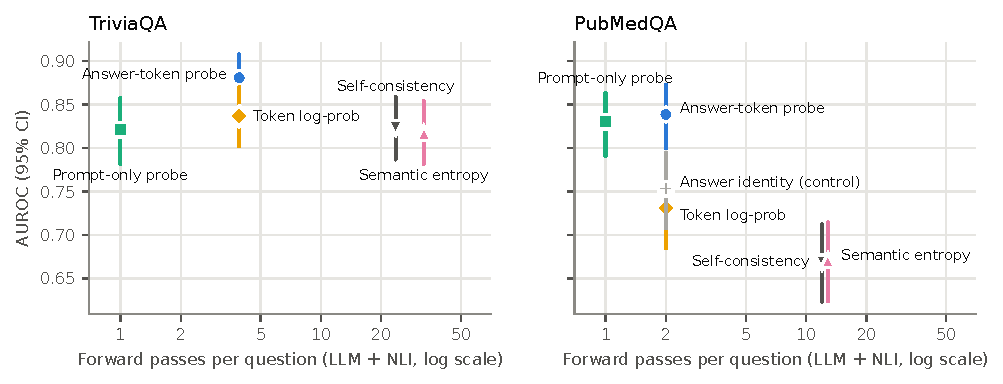
\includegraphics[width=0.82\textwidth]{../figures/fig3_cost_vs_auroc.pdf}
\caption{Cost vs.\ detection quality (3B). Probes need 1--4 forward passes per question;
10-sample self-consistency and semantic entropy need an order of magnitude more.}
\label{fig:cost}
\end{figure*}

\textbf{Probes beat stronger sampling baselines at a fraction of the cost.}
Table~\ref{tab:main} and Fig.~\ref{fig:cost}. The answer-token probe is best on both datasets.
On TriviaQA it improves on 10-sample SE by \TqDProbeAnsvsSEten{} \TqDCiProbeAnsvsSEten{}
and on 10-sample self-consistency by \TqDProbeAnsvsSCten{} \TqDCiProbeAnsvsSCten{}. On
PubMedQA the gaps are \PmDProbeAnsvsSEten{} and \PmDProbeAnsvsSCten{}. Its added latency is
\TqOverProbeAns{}\,ms (TriviaQA), versus \TqOverSEten{}\,ms for 10-sample SE. Ten samples
help the sampling methods (SE: \TqAucSEfive{}$\to$\TqAucSEten{} on TriviaQA), and lenient
clustering changes little; the probe's advantage remains. Over five random splits the
answer-token probe scores \TqRobProbeAns{} (TriviaQA) and \PmRobProbeAns{} (PubMedQA).
Shuffled-label controls (200 permutations) average \TqShufProbeAns{} (TriviaQA) and
\PmShufProbeAns{} (PubMedQA).

\textbf{Hallucinations are predictable before answering.} From the last prompt token
alone (one forward pass, no decoding), the probe reaches \TqAucProbePrompt{} on TriviaQA.
That is statistically indistinguishable from 10-sample SE ($\Delta$ \TqDProbePromptvsSEten{}
\TqDCiProbePromptvsSEten{}) at \TqMsProbePrompt{}\,ms versus \TqMsSEten{}\,ms. On PubMedQA it
reaches \PmAucProbePrompt{}. Caveat: the last prompt token's final layer produces the first
answer token; for PubMedQA's one-word answers, ``before answering'' means before the answer
is emitted, not before it is decided, and the long abstract makes the saving small
(\PmMsProbePrompt{} vs.\ \PmMsLogProb{}\,ms).

\textbf{Controlling for answer identity (PubMedQA).} Error rates depend strongly on the
word chosen, so predicting errors from the yes/no/maybe word alone (cross-fitted) already
gives \PmAucAnsId{}. The probes exceed this control ($\Delta$ \PmDProbeAnsvsAnsId{}
\PmDCiProbeAnsvsAnsId{}). The extra signal lies mostly within ``no'' answers
(prompt probe \PmWithinNoProbePrompt{}, $n{=}\PmWithinNoN$); within ``yes'' the answer
probe is at chance (\PmWithinYesProbeAns{}) and below token log-prob (\PmWithinYesLogProb{}).

\begin{table}[t]
\centering\scriptsize
\begin{tabular}{llccc}
\toprule
Setting & Token & Accuracy probe & SEP & $\Delta$ [95\% CI] \\
\midrule
TriviaQA (in-domain) & prompt & 0.772 & 0.759 & +0.013 [-0.021, +0.052] \\
TriviaQA (in-domain) & answer & 0.821 & 0.784 & +0.037 [-0.003, +0.079] \\
PubMedQA (in-domain) & prompt & 0.793 & 0.752 & +0.041 [+0.007, +0.075] \\
PubMedQA (in-domain) & answer & 0.842 & 0.754 & +0.088 [+0.046, +0.130] \\
TriviaQA $\to$ PubMedQA & prompt & 0.533 & 0.599 & -0.066 [-0.123, -0.010] \\
TriviaQA $\to$ PubMedQA & answer & 0.743 & 0.642 & +0.101 [+0.063, +0.142] \\
PubMedQA $\to$ TriviaQA & prompt & 0.469 & 0.473 & -0.004 [-0.066, +0.059] \\
PubMedQA $\to$ TriviaQA & answer & 0.612 & 0.721 & -0.108 [-0.174, -0.040] \\
\bottomrule
\end{tabular}

\caption{Accuracy probes vs.\ SE probes (SEP; target: binarized 10-sample SE),
both trained on the same 500 questions per dataset. $\Delta$ = accuracy $-$ SEP.}
\label{tab:sep}
\end{table}

\textbf{Accuracy probes vs.\ SE probes.} At matched training data (Table~\ref{tab:sep}),
accuracy probes match or beat SEPs in-domain (answer token: \SepInTqAnsD{} on TriviaQA,
\SepInPmAnsD{} on PubMedQA). Out of domain the picture is mixed and direction-dependent.
For the answer-token probe, PubMedQA$\to$TriviaQA favours the SEP (\SepTrPmTqAnsD{}
\SepTrPmTqAnsDCi{}), in line with \citet{kossen2024sep}, while TriviaQA$\to$PubMedQA favours
the accuracy probe (\SepTrTqPmAnsD{} \SepTrTqPmAnsDCi{}).

\textbf{Cross-domain transfer is fragile.} With the layer chosen on source validation data,
TriviaQA$\to$PubMedQA reaches \TrTqtoPmProbePrompt{} (prompt) and \TrTqtoPmProbeAns{}
(answer token), versus \PmTestProbePrompt{} and \PmTestProbeAns{} in-domain;
PubMedQA$\to$TriviaQA is near chance for the prompt probe (\TrPmtoTqProbePrompt{}). A sweep
over layers shows transfer AUROC for the TriviaQA-trained answer probe ranging from
\TrSweepTqtoPmProbeAnsMin{} to \TrSweepTqtoPmProbeAnsMax{} on PubMedQA. The layer that is best
in-domain (\TrSweepTqtoPmProbeAnsSel{}) is not the one that transfers best
(\TrSweepTqtoPmProbeAnsBest{}), so source-only model selection is unreliable.

\begin{table}[t]
\centering\scriptsize
\begin{tabular}{lcccc}
\toprule
 & \multicolumn{2}{c}{TriviaQA} & \multicolumn{2}{c}{PubMedQA} \\
\cmidrule(lr){2-3}\cmidrule(lr){4-5}
 & 3B & 7B (4-bit) & 3B & 7B (4-bit) \\
\midrule
Model accuracy & 42.6\% & 53.2\% & 61.6\% & 62.1\% \\
\midrule
Answer-token probe (ours) & 0.881 & 0.889 & 0.839 & 0.870 \\
Prompt-only probe (ours) & 0.821 & 0.824 & 0.830 & 0.852 \\
Token log-prob (mean) & 0.837 & 0.846 & 0.731 & 0.519 \\
Self-consistency, 10 samples & 0.845 & 0.840 & 0.698 & 0.616 \\
Semantic entropy, 10 samples & 0.833 & 0.830 & 0.701 & 0.615 \\
\bottomrule
\end{tabular}

\caption{3B vs.\ 7B (4-bit NF4): accuracy and AUROC on the same 500 questions.}
\label{tab:scale}
\end{table}

\textbf{The findings hold at 7B (4-bit).} With the same questions, prompts and protocol
(Table~\ref{tab:scale}), Qwen2.5-7B-Instruct answers \SvTqAcc\% of TriviaQA questions
correctly. The answer-token probe again beats 10-sample SE on TriviaQA
(\SvTqDProbeAnsvsSEten{} \SvTqDCiProbeAnsvsSEten{}). It also beats the answer-identity
control on PubMedQA (\SvPmDProbeAnsvsAnsId{} \SvPmDCiProbeAnsvsAnsId{}). The prompt-only
probe again ties SE on TriviaQA (\SvTqDProbePromptvsSEten{} \SvTqDCiProbePromptvsSEten{}).
On PubMedQA the 7B model hedges with ``maybe'' more often than the gold labels warrant, and
it is about as confident when hedging as otherwise. Token log-prob therefore falls to near
chance (\SvPmAucLogProb{}), while answer identity reaches \SvPmAucAnsId{}. Transfer remains
asymmetric: TriviaQA$\to$PubMedQA reaches \SvTrTqtoPmProbeAns{} for the answer-token probe,
PubMedQA$\to$TriviaQA only \SvTrPmtoTqProbeAns{}.

\section{Limitations}
Two datasets and short answers: SE was designed for, and may be stronger on, longer
generations, and we used at most 10 samples. Labels come from string matching. TriviaQA
aliases include noisy Wikipedia redirects (false positives), and formatting differences
cause false negatives; this label noise is not quantified. PubMedQA test splits are small
(\PmTestN{} questions), so its CIs are wide. The PubMedQA prompt was chosen from the
answer distribution on \PilotN{} questions that are also evaluation questions. Probes need correctness labels in-domain. The 7B
replication uses 4-bit weights, which may perturb hidden states. Results are for one model
family.

\section{Conclusion}
On a single consumer GPU, a linear probe on one hidden state is a stronger and two orders
of magnitude cheaper hallucination detector than 10-sample semantic entropy for short-form
QA, and the prompt alone carries most of that signal. The probe's weak points are equally
clear: it needs in-domain labels, and its cross-domain transfer is fragile. Code, cached
outputs and every number in this paper are generated from one repository.

{\small
\bibliographystyle{plainnat}
\bibliography{references}
}

\appendix
\section{Additional figures}
\begin{figure}[h]
\centering
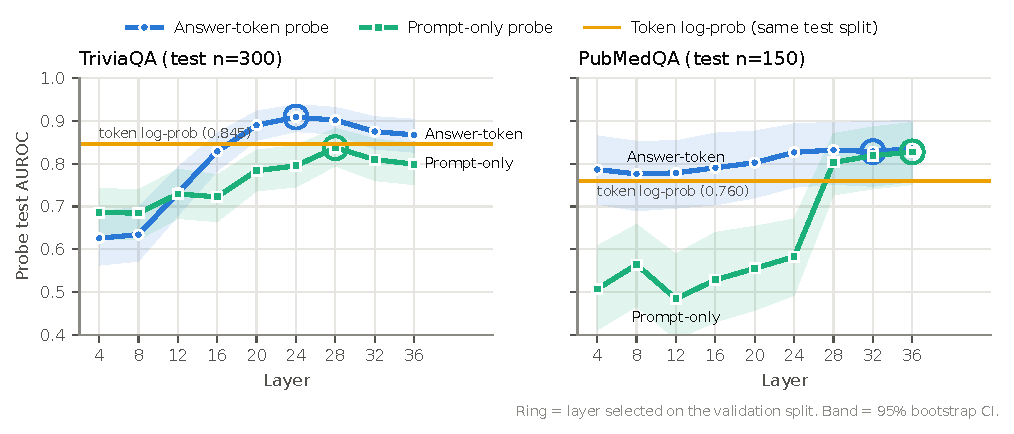
\includegraphics[width=\columnwidth]{../figures/fig4_layer_sweep.pdf}
\caption{Probe test AUROC by layer (3B, fixed split). Ring: layer chosen on validation.}
\end{figure}
\begin{figure}[h]
\centering
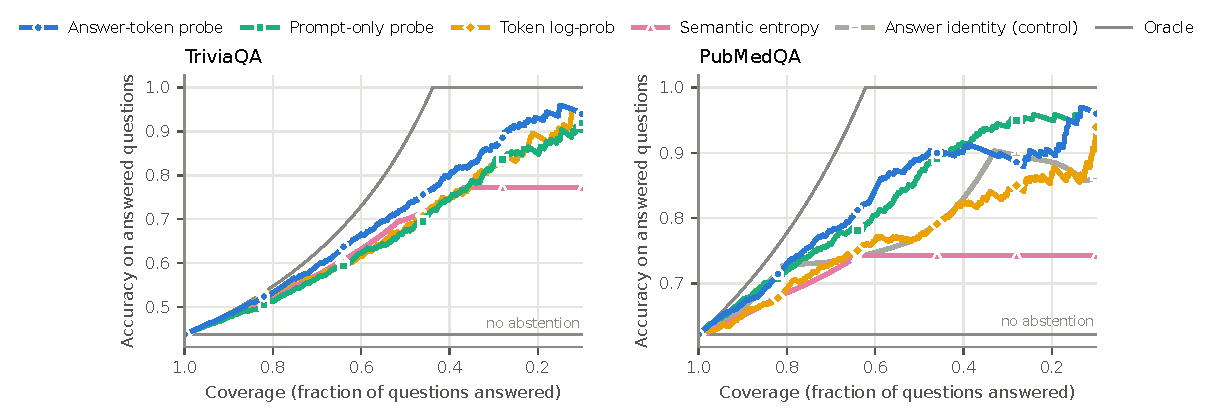
\includegraphics[width=\columnwidth]{../figures/fig2_abstention.pdf}
\caption{Accuracy vs.\ coverage when abstaining on the most uncertain questions.}
\end{figure}
\begin{figure}[h]
\centering
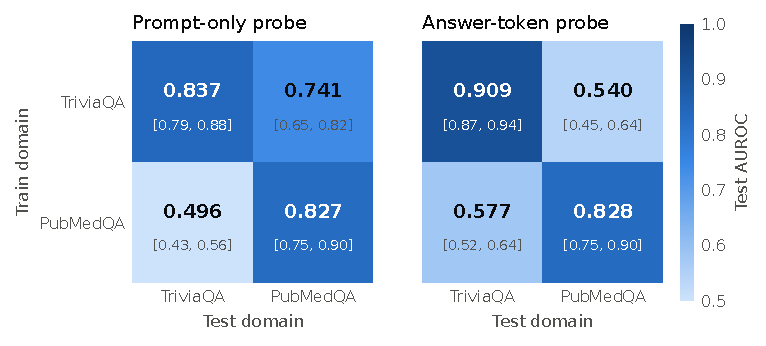
\includegraphics[width=0.85\columnwidth]{../figures/fig5_transfer.pdf}
\caption{Cross-domain transfer (test AUROC), layer chosen on the source validation split.}
\end{figure}

\end{document}
